\documentclass[a4paper,10pt]{article}
\usepackage[margin=3cm]{geometry}
\usepackage{amsmath}
\usepackage{fancyhdr}
\usepackage{hyperref}
\usepackage{graphicx}
\usepackage{float}
\usepackage{algorithm2e}
\usepackage{listings}
%opening
\pagestyle{fancy}{
\fancyhf{}
\fancyhead[L]{\textit{Leone, Micucci, Petocchi}}
\fancyhead[R]{\textsc{\nouppercase{\leftmark}}}
\cfoot{\thepage}
}
\title{Wireless Communications project: comparison of different beamforming techniques in a mobile communication system}
\author{Giuseppe Leone, 10518770 \\ Andrea Micucci, \\ Alessandro Petocchi, 10661410}
\setcounter{tocdepth}{2}

\begin{document}

\maketitle
%\thispagestyle{empty}
\begin{abstract}
In this project we implemented, using the MATLAB language and its toolboxes, a mobile communication system. We analyzed the impact of two different beamforming techniques: the Direction of Arrival (DoA) and the Least Mean Squares (LMS) algorithm in presence of multipath fading. Finally, comparisons between the two methods are presented.
\end{abstract}
%\tableofcontents
\section{Scenario description}
The communication system is made by a Base Station (BS), positioned at a height, and by four terminals situated on the ground. Two of the terminals are the User Equipments (UEs) whose performance we want to analyze, while the other two are interferers. 
The terminals are free to move on the map. Movement is modeled by updating the UEs' coordinates in a while cycle: in each iteration the beamforming operations are performed. Both the distance traveled and the movement direction are random.
\subsection{Communication equipment and modulation}
The BS employs a 4x4 Uniform Rectangular Array (URA) of antennas. Each antenna is spaced by a distance equal to half a wavelength. The UEs transmit the signals and they have one antenna. The terminals employ an OFDM modulation with the following parameters:
\begin{itemize}
	\item FFTLength = 64 (i.e. the total number of sub-carriers)
	\item Guard band sub-carriers = 2 (located at the beginning and at the end of the spectrum)
	\item Pilot sub-carriers = 2 (adjacent to the guard band ones)
	\item Cyclic prefix length = FFTLength/2
	\item Modulation transported: 8-QAM
\end{itemize}
The OFDM parameters are located in the \texttt{OFDMSignal.m} function and can be freely modified: the modulation order is otherwise specified in the main scripts.

\section{Channel models}
This project employs two channel models:
\begin{itemize}
	\item \textbf{Line of Sight (LoS):} this model is used for the DoA beamforming and comparisons with LMS. Attenuation follows the free-space model, i.e. $ \displaystyle L= \left( \frac{4\pi d}{\lambda} \right)^2$. The channel is additionally characterized by the presence of AWGN.
	\item \textbf{QuaDriGa Channel Model:} it is a 3GPP compliant channel model used for characterizing systems affected by multipath fading. In this project it is used for the LMS beamforming algorithm (no DoA is available).The channel is generated as follows:
	\begin{enumerate}
		\item At the start of the iteration, a track for the UEs is defined as stated before.
		\item Channel coefficients and delay taps are calculated for each terminal.
		\item To obtain the channel in the track we perform the interpolation between the delay taps and the transmitted signal: the result is then multiplied by the channel coefficient
		\item The four signals of each terminal are summed into a unique channel and AWGN is added.
		
	\end{enumerate}
\end{itemize}

For both models, the channel is calculated again at each iteration.
\begin{figure}
	\centering
	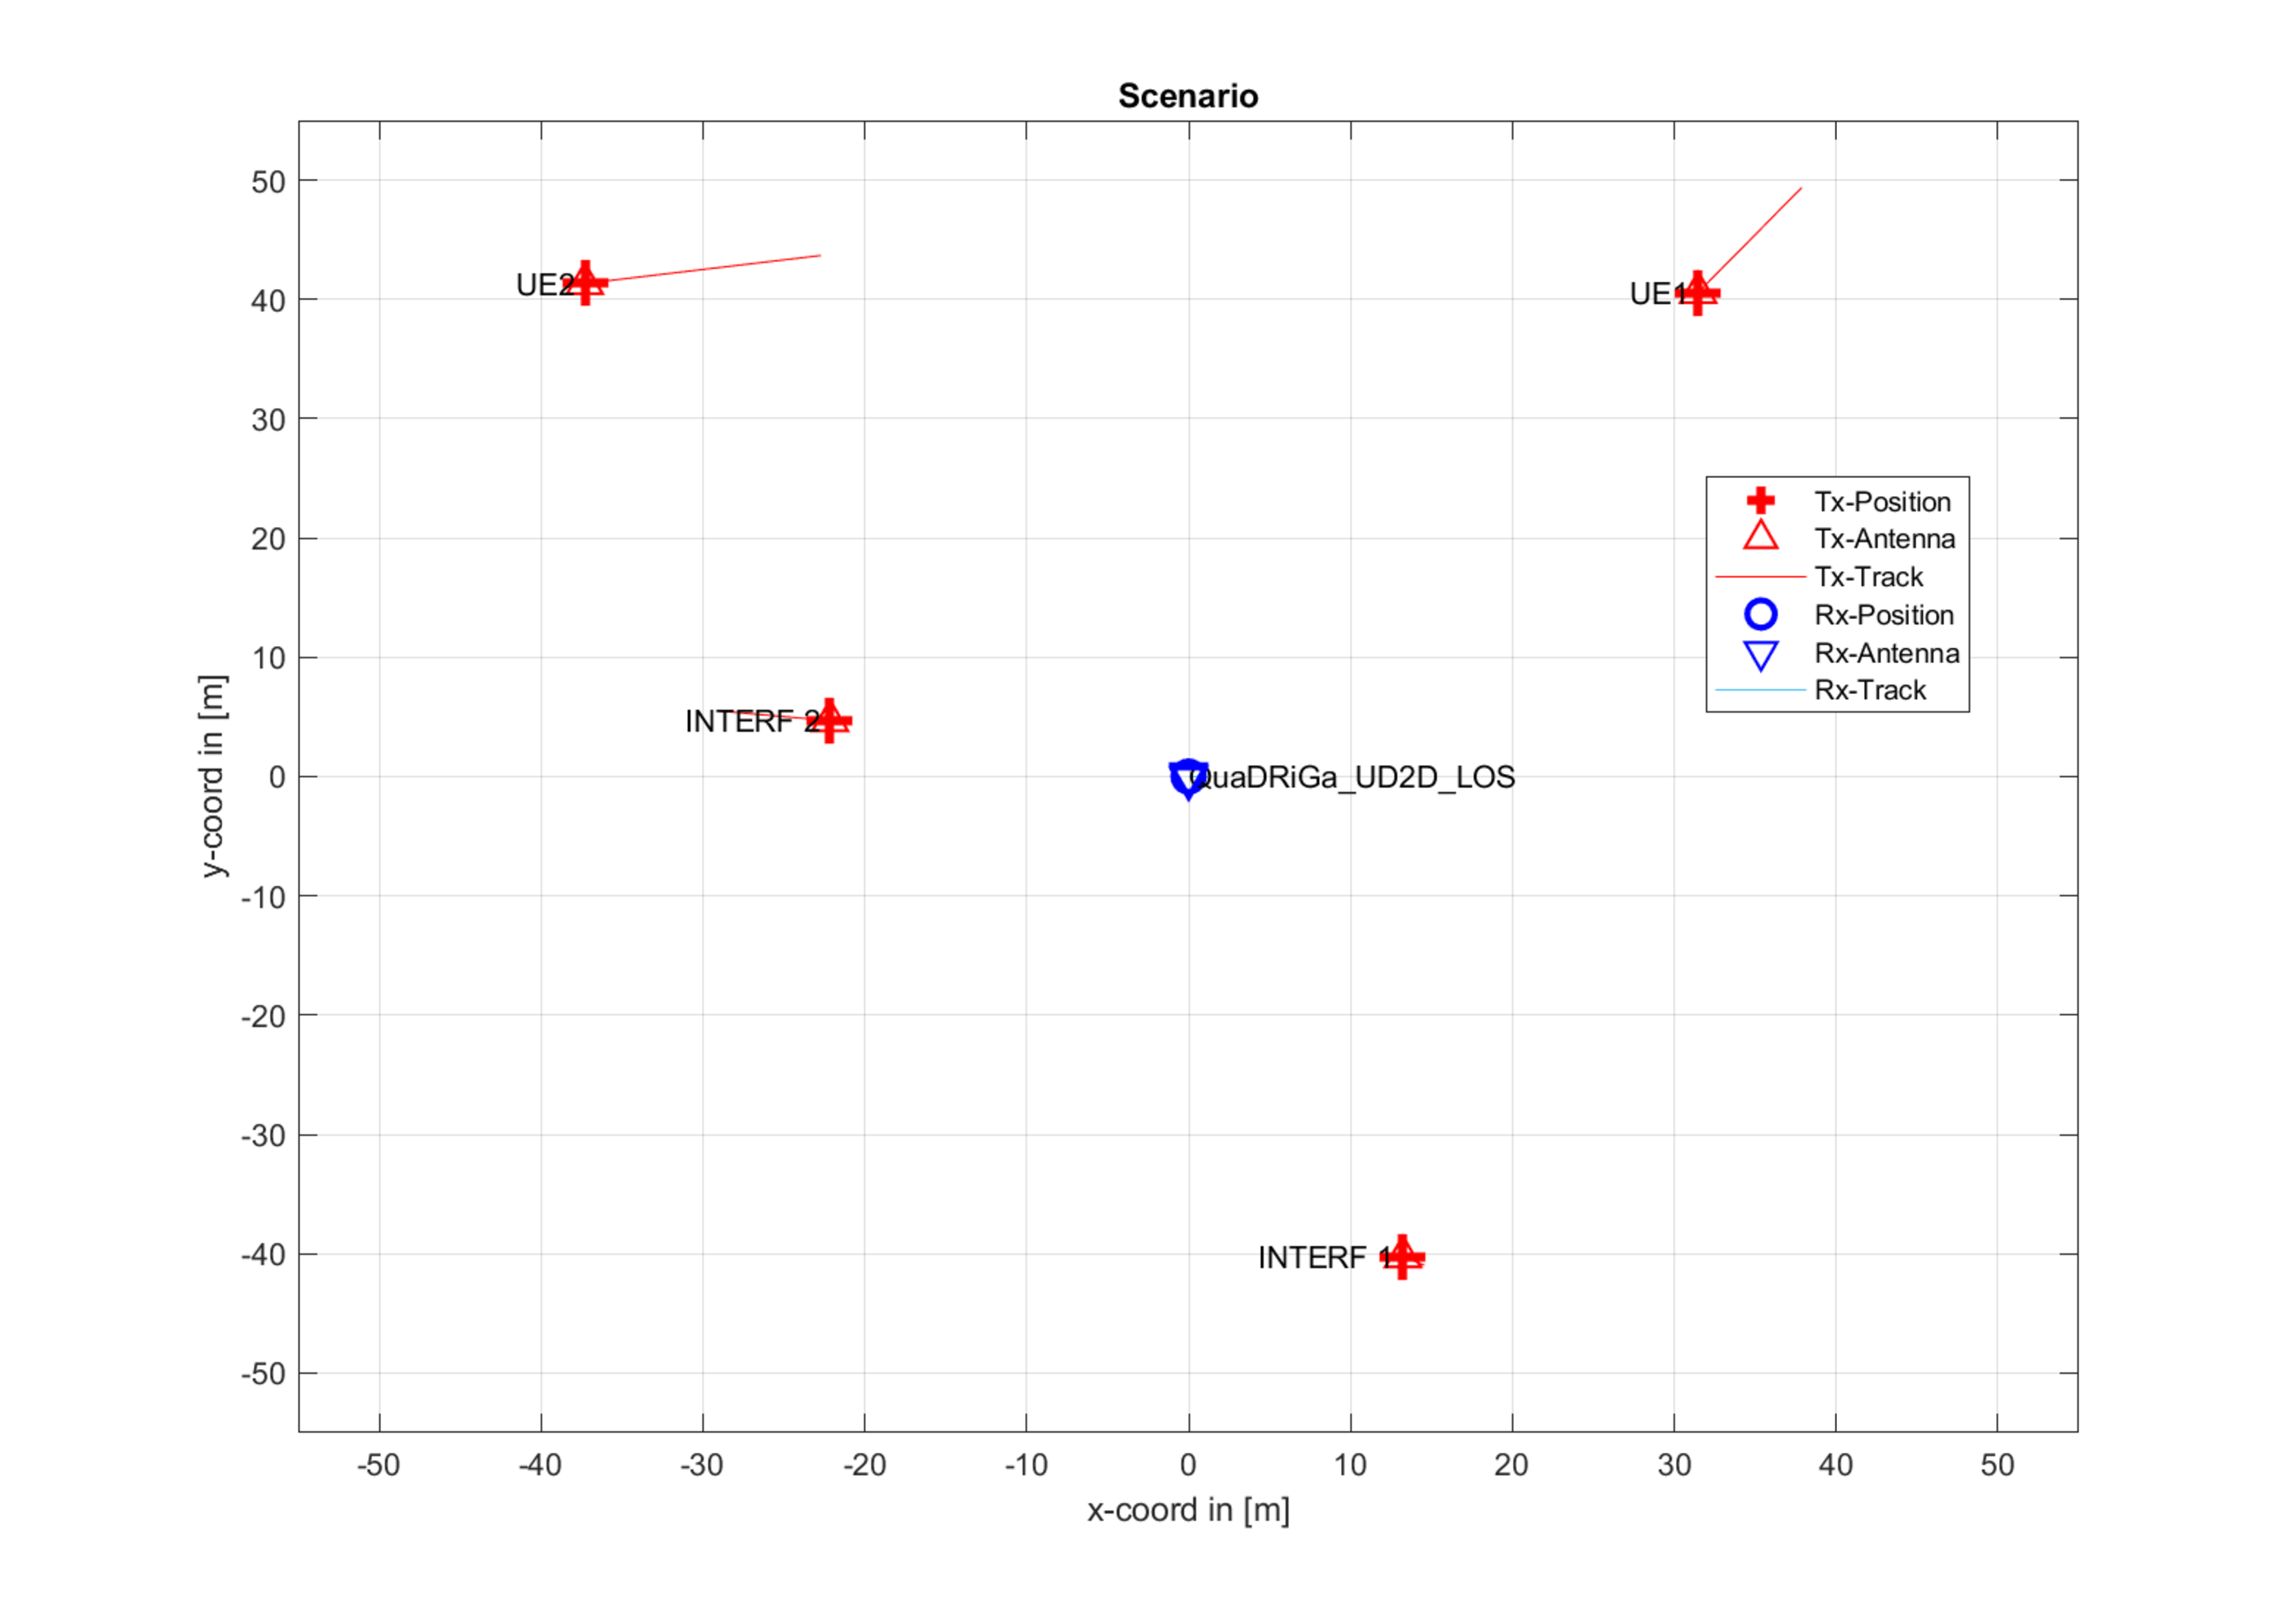
\includegraphics[width=0.8\linewidth]{scenario.pdf}
	\caption{\label{fig:scenario}A bird's-eye visual representation of the scenario}
\end{figure}
\section{LMS beamforming}
Given the transmitted signal $\mathbf{r}$, the channel matrix $\mathbf{C_{out}}$ and the received signal $\mathbf{u}$, from a mathematical point of view the LMS algorithm calculates the weight vector $\mathbf{w}$ as follows:

$$ \mathbf{w_{n+1}} = \mathbf{w_{n}}-\frac{1}{2}\mu \mathbf{\widehat{\nabla}_w MSE}(\mathbf{w})|_{\mathbf{w=w_n}} $$

with $$\mathbf{\widehat{\nabla}_w MSE}(\mathbf{w})|_{\mathbf{w=w_n}} = 2\mathbf{u_n}e_n$$ 
where $e_n = r_n - u_n$ is the error between the transmitted signal and the received one.

\noindent $\mu$ is the gradient step size and is defined as $\displaystyle \mu = \frac{2}{\mathrm{Tr}(\mathbf{C_{out}})}$ \\

The MATLAB implementation of this algorithm may be found in the \texttt{LMSalgorithm.m} function file. Given a sample of the transmitted signal, at each iteration the error between the transmitted sample and the received sample is calculated, where the received sample is given by a weighted sum of the samples received from each antenna in the URA. The weights are the ones that were calculated in the previous iteration. 

After evaluating the error, the weights are updated according to the formula described above. This operation is performed for all of the samples contained in the received signal vector.

The algorithm is employed for beamforming in the script \texttt{LMSQuadriga.m} . After the scenario and channel setup, the weight vector is calculated. The script then proceeds to multiply the signals received from the two tracked UEs with it, thus completing the beamforming procedure. Then, a comparison between the BER calculated with and without LMS BF is performed for different values of the SNR.

\begin{figure}[H]
	\centering
	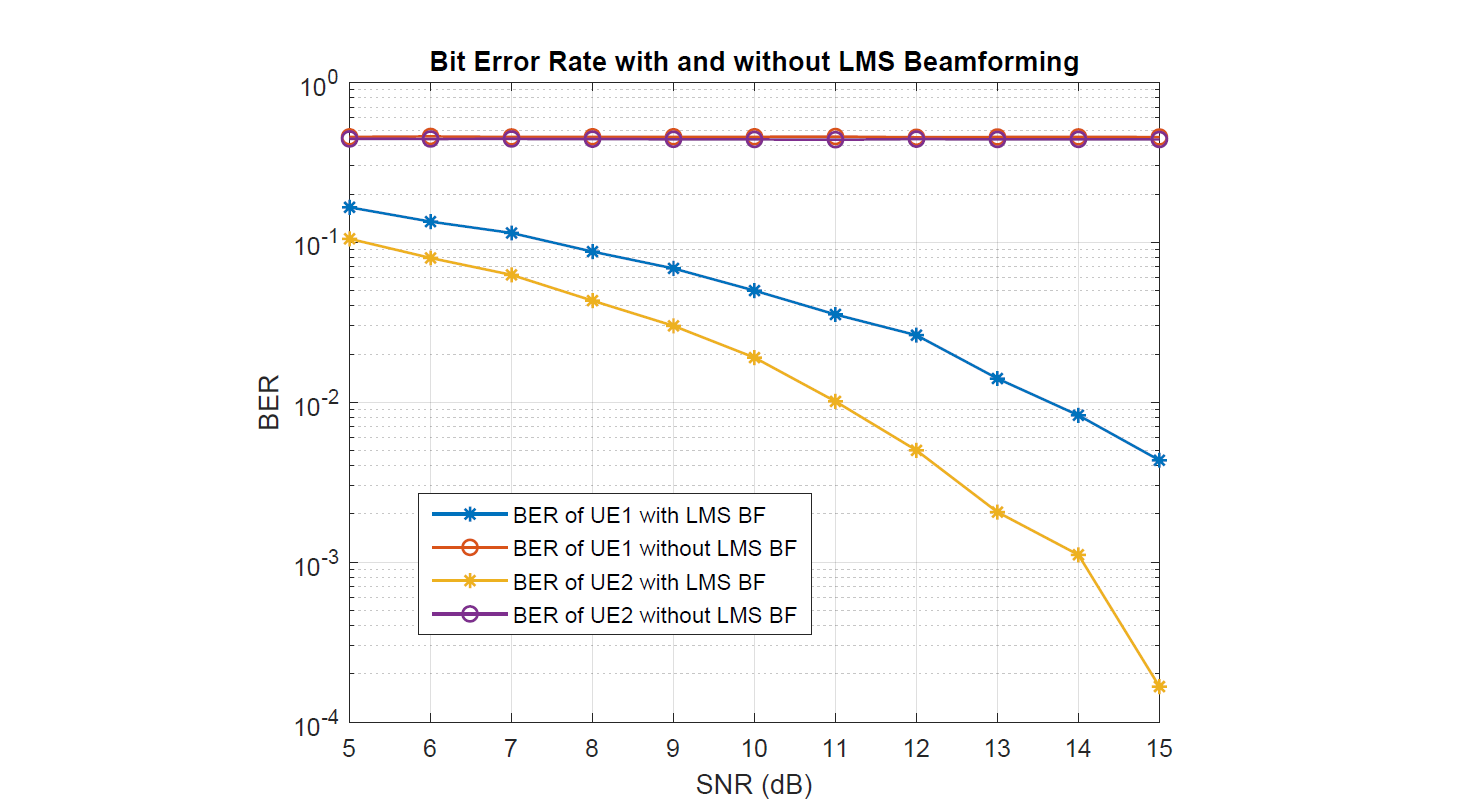
\includegraphics[width=\linewidth]{bersnr.png}
	\caption{\label{fig:bersnr}Results of the comparisons for different SNRs.}
\end{figure}
As we can see from Figure \ref{fig:bersnr}, the LMS beamforming dramatically improves performance, in particular for high values of SNR.
\section{Direction of Arrival (DoA) beamforming}
\end{document}